\chapter{Applying the coupling}\label{ch:c7}
This chapter takes the user from data to a calibrated coupled model: a complete worked example with the Liard River model,
how to prepare data for another basin, a checklist and typical parameter values, calibration, and troubleshooting.

\begin{plain}
This chapter walks through a real example --- the Liard River in northern Canada --- from input files to results. It then
shows how to set up your own watershed, which values to start from, how to calibrate, and what to do when something goes
wrong.
\end{plain}

\section{Tutorial: the Liard River model}\label{ch:tutorial}
This chapter walks through the example supplied in \cmd{examples/Liard\_groundwater}: the Liard River model (65 subbasins,
1\,107 HRUs, northern British Columbia and Yukon) with an aquifer added under three nested subbasins (52, 48 and 43;
about 13\,800 km$^2$, 85 coupled HRUs). The other 62 subbasins run exactly as before.

\subsection{Step 0: prepare}
\begin{enumerate}
\item Build Raven from this source (CMake: \cmd{mkdir build; cd build; cmake ..; make}; or \cmd{make} in \cmd{src/}; on Windows open \cmd{src/Raven.sln}).
\item Get the MODFLOW~6 library (6.5 or newer; tested with 6.8.1 and 6.6.3; 6.8 or newer recommended): run
\cmd{python tools/get\_mf6.py} in the source folder, or build with CMake, which fetches it (Section~\ref{sec:getmf6}).
Raven then finds it without any setting.
\item The original Liard package was made for Raven 2.9.1; for Raven 4.x its Windows paths use \texttt{/} and the parameter
\cmd{DEP\_THRESHHOLD} is spelled \cmd{DEP\_THRESHOLD}. The example files already include these changes.
\end{enumerate}

\subsection{Step 1: mark the HRUs with groundwater (.rvh)}
In the \cmd{:HRUs} table, the \cmd{AQUIFER\_PROFILE} column was filled for the HRUs of subbasins 52, 48 and 43:
\cmd{VALLEY\_ALLUVIUM} for forest, shrub and wetland HRUs; \cmd{UPLAND\_TILL} for barren HRUs; glaciers keep \cmd{[NONE]}.
A group listing the same HRUs was added at the end of the file:
\par\noindent\begin{minipage}{\linewidth}
\begin{lstlisting}
:HRUGroup AquiferHRUs
  2736, 2745, 2747, ...
:EndHRUGroup
\end{lstlisting}
\end{minipage}\par\smallskip

\subsection{Step 2: describe the aquifer (.rvp)}
Added at the end of \cmd{Liard.rvp}:
\begin{lstlisting}
:AquiferClasses
  :Attributes, K_HORIZ, K_VERT, SPEC_STORAGE, SPEC_YIELD, POROSITY
  :Units,      m/d,     m/d,    1/m,          none,       none
  GRAVEL,      50.0,    5.0,    1.0E-5,       0.25,       0.30
  CLAY_TILL,   0.001,   0.0001, 1.0E-4,       0.03,       0.40
  SAND,        10.0,    1.0,    1.0E-5,       0.20,       0.35
  UPLAND_TILL, 0.2,     0.02,   1.0E-4,       0.08,       0.30
:EndAquiferClasses

:AquiferProfiles
  VALLEY_ALLUVIUM, 3, GRAVEL, 15.0, AQUIFER, CLAY_TILL, 5.0, AQUITARD, SAND, TO_BEDROCK, CONFINED_AQUIFER
  UPLAND_TILL,     1, UPLAND_TILL, TO_BEDROCK, AQUIFER
:EndAquiferProfiles

:AquiferProfileParameters
  :Attributes,     INITIAL_HEAD_DEPTH, DEFAULT_BEDROCK_DEPTH, SEEPAGE_LEAKANCE, SOIL_ZONE_DEPTH
  :Units,          m,                  m,                     1/d,              m
  VALLEY_ALLUVIUM, 3.0,                60.0,                  1.0,              0.0
  UPLAND_TILL,     8.0,                15.0,                  1.0,              0.0
:EndAquiferProfileParameters
\end{lstlisting}
The valley aquifer is a gravel layer (15 m) over a clay-till aquitard (5 m) over sand down to bedrock; the uplands have one
till layer to shallow bedrock.

\subsection{Step 3: switch the coupling on and send recharge to it (.rvi)}
\par\noindent\begin{minipage}{\linewidth}
\begin{lstlisting}
:GroundwaterModel MODFLOW6
:DefineHRUGroups AquiferHRUs
...
:Percolation PERC_CONSTANT FAST_RESERVOIR SLOW_RESERVOIR
  :-->Conditional HRU_GROUP IS_NOT AquiferHRUs     # existing process, now only for uncoupled HRUs
:Percolation PERC_CONSTANT FAST_RESERVOIR GROUNDWATER
  :-->Conditional HRU_GROUP IS AquiferHRUs         # new: this water becomes recharge
\end{lstlisting}
\end{minipage}\par\smallskip
Seepage returns to the lowest soil layer (\cmd{SLOW\_RESERVOIR}), whose existing baseflow process carries it to the rivers;
aquifer--river exchange goes directly to the reaches.

\subsection{Step 4: the groundwater file (.rvg)}
\begin{lstlisting}
#########################################################################
# Liard.rvg - Raven-MODFLOW 6 groundwater file (Liard River test case)
#   Groundwater under Central Liard subbasins 52 -> 48 -> 43 (85 HRUs).
#   Hydrogeology (aquifer classes, profiles) is in Liard.rvp;
#   which HRUs have groundwater is set by AQUIFER_PROFILE in Liard.rvh.
#########################################################################

# --- geometry (stand-in data built by tools_build_standin_inputs.py; replace with real data) ---
:HRUGeometry        Liard_HRUs_standin.geojson  HRU_ID    # HRU polygons, lon/lat
:RiverGeometry      Liard_rivers.geojson                  # river lines (subbasin assigned automatically)
:LandSurface        Liard_dem_standin.asc                 # DEM, ESRI ASCII, lon/lat
:BedrockSurface     Liard_bedrock_standin.asc             # bedrock elevation, same format

# --- grid and coupling settings ---
:GridCellSize       2000.0     # m
:MinCellCoverage    0.25       # fraction of a cell covered by coupled HRUs to activate it
:HeadSaveFrequency  365        # steps between saves of the full head field (mf6/gwf.hds)
# :MF6Library       /path/to/libmf6.so    # only for a library outside lib/mf6/ (or RAVEN_MF6_LIB)

# --- optional features (uncomment to use; see the user guide) ---
# :GWInitialization  STEADY_STATE 0.45            # steady-state start, uniform recharge [mm/d]
# :SurfaceWaterExchange DEPRESSION WetlandHRUs LEAKANCE 0.01   # wetlands <-> aquifer
# :WriteNetCDFHeads                               # GWHeads.nc (Raven built with -Dnetcdf)
# :ReservoirExchange                              # Raven reservoirs (with :SeepageParameters) <-> aquifer
# :Wells
#   :Attributes, NAME, LATITUDE, LONGITUDE, SCREEN_TOP, SCREEN_BOT
#   1, PW_1, 59.27310, -124.73460, 1199.7, 1188.7
# :EndWells                                        # rates: :WellRate 1 m3/d ... in Liard.rvt
# :ObservationWells
#   :Attributes, NAME, LATITUDE, LONGITUDE, SCREEN_ELEV
#   101, OW_NEAR, 59.27310, -124.73060, 1192.7
# :EndObservationWells                             # data: :ObservationData GW_HEAD 101 m ... in Liard.rvt
# :GeneralHeadBoundary   GHB1 boundary_line.geojson HEAD 1146.85 CONDUCTANCE 5000.0 LAYERS TOP
# :SpecifiedHeadBoundary LAKE1 lake.geojson HEAD 1226.5 LAYERS TOP
\end{lstlisting}
The HRU polygons, DEM and bedrock of this example are \emph{stand-ins}: the Liard package has no HRU polygons, DEM or
bedrock map, so \cmd{tools\_build\_standin\_inputs.py} made Voronoi polygons around the HRU centroids clipped to each
subbasin, a DEM interpolated from HRU elevations, and bedrock 60 m (valley), 15 m (upland) and 5 m (glacier) below it.
For a real study, replace them with real data.

\subsection{Step 5: run}
\par\noindent\begin{minipage}{\linewidth}
\begin{lstlisting}
cd examples/Liard_groundwater
../../Raven.exe Liard -o output/
python3 tools_audit.py output        # optional automated check
\end{lstlisting}
\end{minipage}\par\smallskip
The 20-year daily run takes about 15 minutes on one processor core (35 seconds without groundwater). Raven builds a grid of
3 layers $\times$ 85 $\times$ 54 cells of 2 km, 3\,252 active columns, 178 river cells (Figure~\ref{fig:grid}).

\subsection{Step 6: look at the results}
\begin{itemize}
\item \cmd{GWModelSummary.txt}: check the grid, the number of active cells and that every coupled HRU is linked.
\item \cmd{GWBudget.csv}: the daily groundwater balance (Figure~\ref{fig:budget}); the error column should stay tiny.
\item \cmd{GWHRUState.csv}: depth to water under each HRU (Figure~\ref{fig:wtdepth} shows the map from \cmd{mf6/gwf.hds}).
\item \cmd{Hydrographs.csv}: streamflow now includes groundwater discharge (Figure~\ref{fig:hydro}).
\end{itemize}
\begin{figure}[h]\centering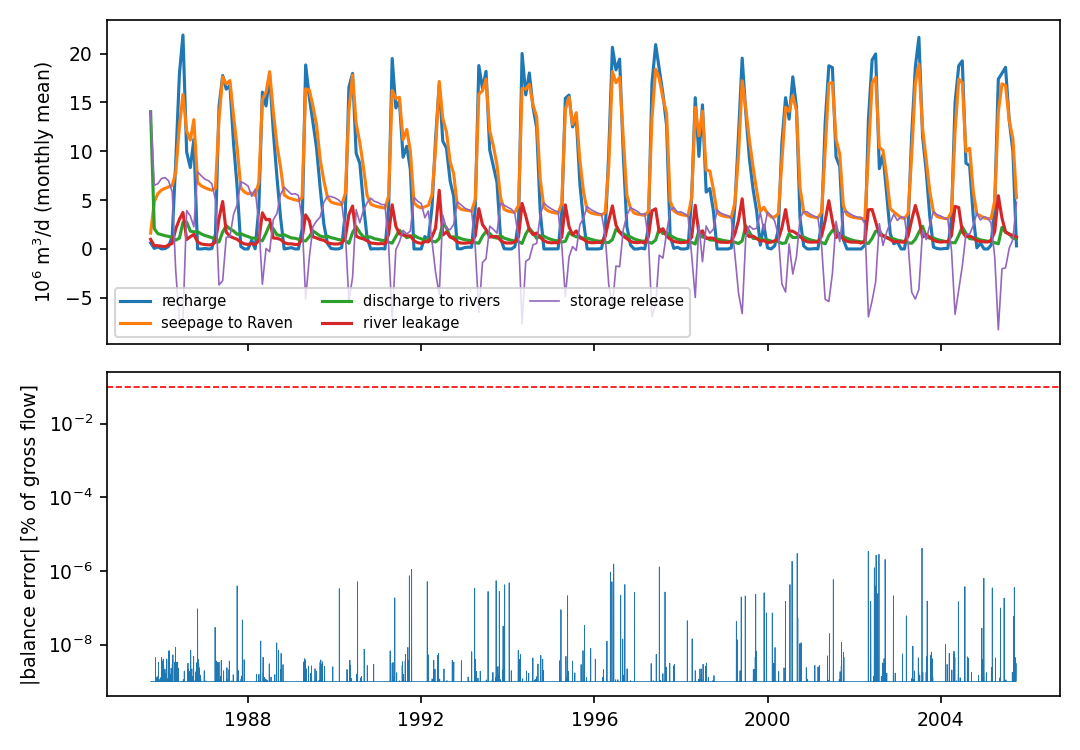
\includegraphics[width=\linewidth]{figures/fig_budget.png}
\caption{Groundwater budget of the 20-year Liard run (monthly means) and daily balance error; the dashed line is 0.1\%.}\label{fig:budget}\end{figure}
\begin{figure}[h]\centering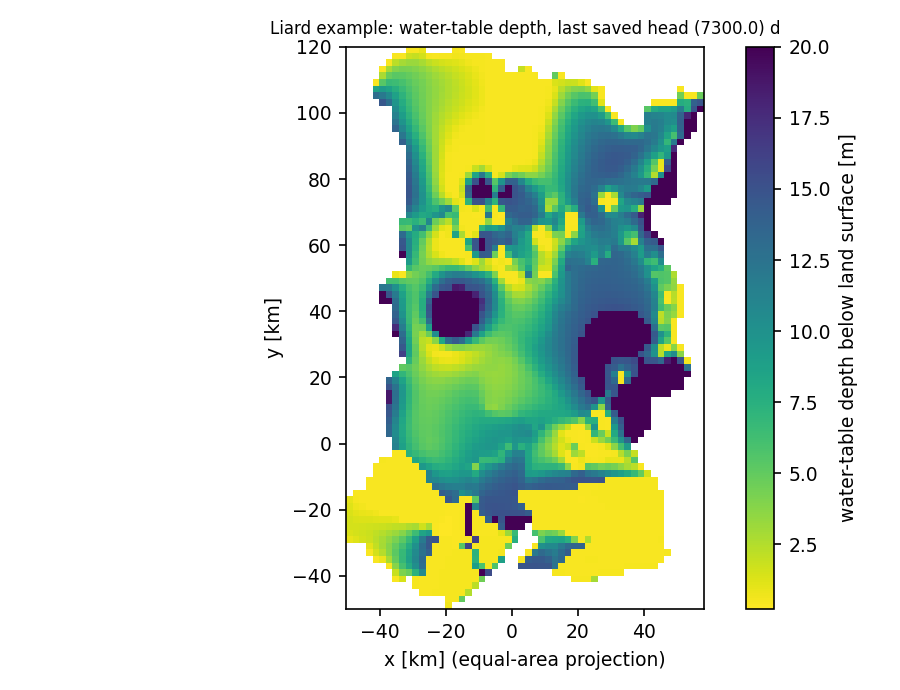
\includegraphics[width=0.72\linewidth]{figures/fig_wtdepth.png}
\caption{Depth to water at the last saved head.}\label{fig:wtdepth}\end{figure}
\begin{figure}[h]\centering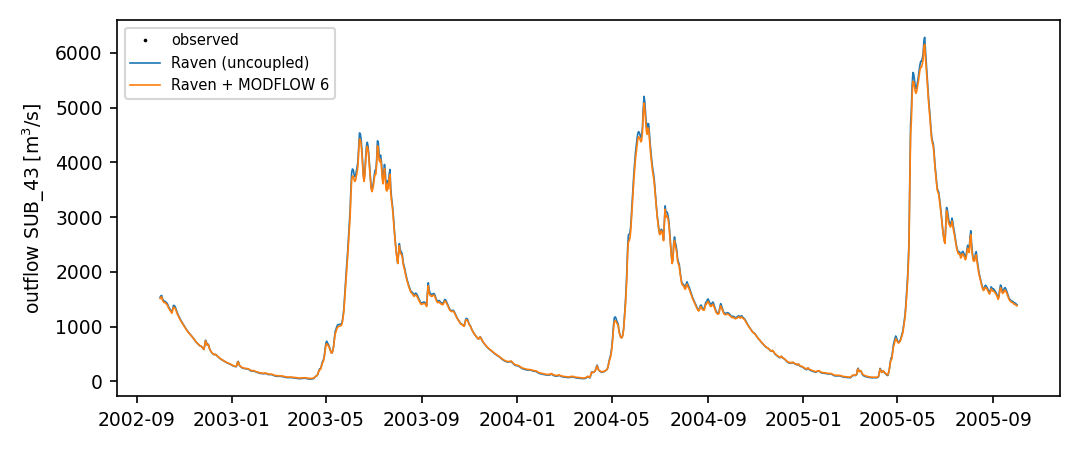
\includegraphics[width=\linewidth]{figures/fig_hydrograph.png}
\caption{Outflow of subbasin 43, 2003--2005, without and with groundwater (not recalibrated).}\label{fig:hydro}\end{figure}
Without recalibration and with stand-in geometry, the Nash--Sutcliffe efficiency at gauges 10BE004, 10BE005 and 10BE010
changes from 0.867, 0.835, 0.681 to 0.850, 0.821, 0.634. Recalibrating with flow and head data is the natural next step.

\section{Preparing the input data}
\subsection{HRU polygons}
Raven's HRUs usually come from a GIS overlay (for example BasinMaker): subbasins intersected with land-use, soil and terrain
classes. Export that polygon layer, keeping the HRU ID used in the \cmd{.rvh}:
\par\noindent\begin{minipage}{\linewidth}
\begin{lstlisting}
ogr2ogr -f GeoJSON -t_srs EPSG:4326 my_hrus.geojson my_hrus.shp
\end{lstlisting}
\end{minipage}\par\smallskip
(or, in QGIS, \emph{Export $\rightarrow$ Save Features As}, format GeoJSON, CRS EPSG:4326). Check that every HRU with an
\cmd{AQUIFER\_PROFILE} appears in the file; \cmd{GWModelSummary.txt} lists, per HRU, its polygon area, its area in the \cmd{.rvh}
and the fraction linked to active cells.
\subsection{Maps}
Convert the DEM and the bedrock (or aquifer base) surface to ESRI ASCII grids in longitude/latitude:
\par\noindent\begin{minipage}{\linewidth}
\begin{lstlisting}
gdalwarp -t_srs EPSG:4326 -tr 0.005 0.005 -r bilinear dem.tif dem_lonlat.tif
gdal_translate -of AAIGrid dem_lonlat.tif dem_lonlat.asc
\end{lstlisting}
\end{minipage}\par\smallskip
Use a raster resolution finer than the model cells (each model cell averages 25 samples). Both maps must use the same
vertical datum, as must well screens, monitoring wells, boundary heads and reservoir stages.
\subsection{River lines}
Any line layer of the river network in longitude/latitude. A field with the Raven subbasin ID is optional; without it, each
river piece is assigned to the subbasin of the HRU that dominates its grid cell.
\subsection{Aquifer information}
Layer thicknesses and materials come from borehole logs, geological maps or regional hydrogeological studies. Start with one or
two profiles and typical values (Section~\ref{ch:ownmodel}); refine only where data or calibration demand it.

\section{Choosing a grid for the Liard model}\label{sec:liardgrids}
The Liard model was run for two years on each grid option (Table~\ref{tab:liardgrids}); every run keeps the water accounts
exact (MODFLOW residual about $10^{-11}$, no failed step, Raven's balance unchanged).
\begin{table}[!htbp]\centering
\caption{The Liard model (2 years) on each grid: active cells, run time on one core, Nash--Sutcliffe efficiency at 10BE004 /
10BE005 / 10BE010, mean seepage to Raven and mean net aquifer discharge to rivers [million m$^3$/d].}\label{tab:liardgrids}
\begin{tabular}{lrrcrr}\toprule\hdr
Grid & Cells & Time [s] & NSE & Seepage & Rivers\\\midrule
Regular 2 km (default) & 8\,840 & 40 & 0.728 / 0.861 / 0.635 & 9.48 & 0.82\\
Regular, rotated 20\textdegree, 1 km along rivers & 35\,058 & 220 & 0.726 / 0.861 / 0.638 & 9.92 & 0.66\\
Quadtree 2 km, 500 m along rivers & 16\,276 & 108 & 0.719 / 0.858 / 0.611 & 9.49 & 0.01\\
HRU mesh 2 km, 1 km along rivers & 14\,610 & 100 & 0.717 / 0.859 / 0.627 & 9.94 & 0.35\\
Regular 2 km, layers by elevation & 8\,840 & 41 & 0.666 / 0.859 / 0.606 & 4.11 & 0.49\\
\bottomrule\end{tabular}
\par\smallskip\footnotesize Final code with MODFLOW 6.8.1 (\cmd{tests/liard\_grids.py}); run times on one core of the test machine.
\end{table}
Streamflow hardly changes: total seepage is nearly the same on every grid and the river exchange is a small part of the
flow at the gauges. The net river exchange, however, depends on the size of the river cells --- 0.82 million m$^3$/d with
2 km cells, 0.01 with 500 m cells --- for two reasons: the channel bed is placed at the lowest DEM value along the river in
each cell, which is lower in larger cells, and the head of a large cell averages the aquifer over a wider area around the
river. Calibrate the riverbed parameters (\cmd{RIVERBED\_K}, \cmd{:RiverBedDepth}) on the grid that will be used, and
compare models only at the same river-cell size. Connecting layers by elevation halves the seepage here, because water in
the upland till can now flow directly into the valley gravel where the two lie at the same elevation --- a different
conceptual model rather than a refinement. A regular grid refined to 1 km along rivers has more than twice the cells of a
quadtree with 500 m river cells, because its refinement spans whole rows and columns.

\section{Setting up your own model}\label{ch:ownmodel}
\subsection{Checklist}
\begin{enumerate}
\item \textbf{HRU polygons.} Export the HRU polygons from your GIS or BasinMaker as GeoJSON in longitude/latitude
(EPSG:4326), with a field holding the HRU ID used in the \cmd{.rvh} file.
\item \textbf{Maps.} A DEM and a bedrock (or aquifer-base) elevation map as ESRI ASCII grids in longitude/latitude, in the same
vertical datum. River lines as GeoJSON.
\item \textbf{Profiles.} Group your HRUs by the aquifer beneath them and write one profile per group; set
\cmd{AQUIFER\_PROFILE} in the \cmd{.rvh}.
\item \textbf{Recharge.} Decide which Raven flux is recharge (usually percolation from the deepest soil store) and send it
to \cmd{GROUNDWATER} for coupled HRUs only. Remove or restrict any process that drains \cmd{GROUNDWATER} there, and any
conceptual baseflow that would double-count groundwater.
\item \textbf{Grid size.} Choose $\Delta$ so that the smallest features you care about span a few cells, but the number of
active cells stays manageable (a few thousand to a few hundred thousand per layer).
\item \textbf{Start.} Use \cmd{:GWInitialization STEADY\_STATE} with the long-term average recharge, or a warm-up period.
\item \textbf{Check.} Read \cmd{GWModelSummary.txt} and run \cmd{tools\_audit.py}.
\item \textbf{Calibrate.} Use streamflow and monitoring-well heads (Section~\ref{ch:calib}).
\end{enumerate}

\section{Typical parameter values}
Typical values for aquifer materials are listed in Section~\ref{app:materials}, and typical ranges for every aquifer class
and profile parameter in Sections~\ref{app:class} and~\ref{app:profile}.

\subsection{How much of the water balance should groundwater take?}
In a coupled HRU, Raven's conceptual baseflow from deep stores is replaced by MODFLOW. Check after a first run that the
long-term baseflow (seepage plus aquifer discharge to rivers) is plausible, and that the aquifer is not steadily filling or
emptying (storage release near zero on average once spin-up is over).

\section{Calibration}\label{ch:calib}
Aquifer class and profile parameters are ordinary entries in the \cmd{.rvp} file, so they can be calibrated with Ostrich
exactly like soil parameters: make a template of the \cmd{.rvp} with parameter names in place of values.
\par\noindent\begin{minipage}{\linewidth}
\begin{lstlisting}
  GRAVEL,      par_K_gravel, 5.0,  1.0E-5, par_Sy_gravel, 0.30
  UPLAND_TILL, par_K_till,   0.02, 1.0E-4, 0.08,          0.30
\end{lstlisting}
\end{minipage}\par\smallskip
Monitoring-well heads (\cmd{:ObservationData GW\_HEAD}) are scored in \cmd{Diagnostics.csv} next to streamflow, so an
objective can combine both. Calibrate conductivities on a logarithmic scale. \cmd{docs/ostrich\_example/} contains an
\cmd{ostIn.txt} using DDS \cite{tolson2007dds}, the template and run scripts. Because the linkage is cached, repeated runs
skip the geometry work.

\subsection{A synthetic test}
Groundwater under subbasin 52 only (545 active columns), 2 years, 7 s per run. Heads from a run with known parameters, plus
2 cm of random noise, at four monitoring wells were the observations. The search started from values 2.5 to 10 times off.
\begin{table}[!htbp]\centering
\caption{Synthetic calibration: the parameters used to make the ``observations'', the starting values, and the values DDS recovered.}\label{tab:synthcal}
\begin{tabular}{lrrrr}\toprule\hdr
Parameter & True & Start & After 150 runs & Error\\\midrule
Gravel $K$ [m/d] & 50 & 5 & 47.7 & $-4.6$\%\\
Gravel $S_y$ & 0.25 & 0.10 & 0.239 & $-4.5$\%\\
Upland-till $K$ [m/d] & 0.2 & 2.0 & 0.149 & $-25$\%\\\bottomrule
\end{tabular}\end{table}
Table~\ref{tab:synthcal} shows the result. The objective (sum of RMSE over the four wells) fell from 14.4 m to 0.17 m (it is 0.08 m at the true values, so more runs
would refine it further; Figure~\ref{fig:calib}). The upland-till conductivity is the hardest to identify because the
upland heads respond weakly to it.
\begin{figure}[h]\centering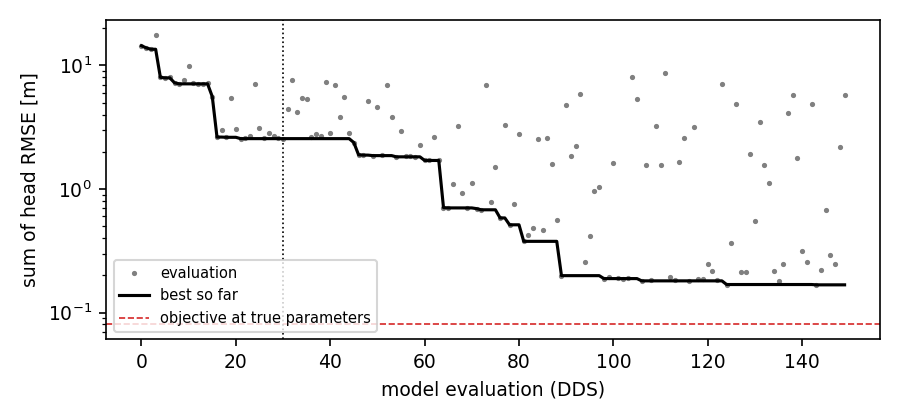
\includegraphics[width=0.8\linewidth]{figures/fig_calibration.png}
\caption{Synthetic calibration: objective against model runs.}\label{fig:calib}\end{figure}

\section{The Ostrich input file, line by line}
\begin{lstlisting}
ProgramType         DDS             # search algorithm (dynamically dimensioned search)
ObjectiveFunction   GCOP            # general constrained optimization
ModelExecutable     ./Ost-Raven.sh  # script that runs Raven in ./model
BeginFilePairs
  Liard.rvp.tpl ; model/Liard.rvp   # template -> model file with values filled in
EndFilePairs
BeginParams                         # name, start, lower, upper, transformations
  par_K_gravel   5.0  1.0  500.0  none log10 none
  par_Sy_gravel  0.10 0.05 0.35   none none  none
  par_K_till     2.0  0.01 5.0    none log10 none
EndParams
BeginResponseVars                   # values read from Diagnostics.csv
  RMSE1  model/output/Diagnostics.csv ; OST_NULL 1 5 ','
  ...
EndResponseVars
BeginTiedRespVars                   # objective = sum of the RMSEs
  SUM_RMSE 4 RMSE1 RMSE2 RMSE3 RMSE4 wsum 1.0 1.0 1.0 1.0
EndTiedRespVars
BeginGCOP
  CostFunction SUM_RMSE
EndGCOP
BeginDDSAlg
  MaxIterations 150
EndDDSAlg
\end{lstlisting}
Check the row and column of each response in your own \cmd{Diagnostics.csv}; they depend on the order of observations and on
\cmd{:EvaluationMetrics}. To combine heads and streamflow, add NSE or KGE responses of the hydrographs with suitable weights.

\section{Troubleshooting}\label{ch:trouble}
\begin{table}[!htbp]\centering
\caption{Messages and symptoms, with their causes and remedies.}
\begin{tabular}{P{0.36\linewidth}P{0.588\linewidth}}\toprule\hdr
Message or symptom & Cause and remedy\\\midrule
``cannot load MODFLOW 6 library'' & run \cmd{python tools/get\_mf6.py} in the source folder, or set \cmd{:MF6Library} or \cmd{RAVEN\_MF6\_LIB} to the full path of \cmd{libmf6}; the message lists the places searched\\
Raven stops during initialization without a Raven message & MODFLOW rejected its input; read \cmd{<output>/mf6/mfsim.lst}\\
``HRU \dots\ has an AQUIFER\_PROFILE but no polygon'' & HRU IDs in the GeoJSON do not match the \cmd{.rvh}; check the ID field name\\
``does not overlap any active groundwater cell'' & the HRU is too small for the grid or sits where bedrock is at the surface; reduce \cmd{:GridCellSize} or \cmd{:MinCellCoverage}, or check the bedrock map\\
``polygon area \dots\ differs from .rvh AREA'' & information only; volumes are always consistent\\
``process \dots\ removes water from GROUNDWATER'' & a Raven process drains \cmd{GROUNDWATER} in a coupled HRU; restrict it with \cmd{:-->Conditional}\\
``process \dots\ sends water to GROUNDWATER in HRU \dots\ which has no AQUIFER\_PROFILE'' & that water would leave the model; restrict the process\\
``MODFLOW 6 did not converge'' & start from a steady state or realistic heads; raise \cmd{:SolverMax\allowbreak OuterIterations}; increase \cmd{SEEPAGE\_SMOOTHING\_DEPTH}; check for extreme parameter contrasts\\
Well rate is zero (``no :WellRate time series'') & the \cmd{:WellRate} block is missing, or its ID does not match an ID in \cmd{:Wells}\\
``reservoir \dots\ has no :SeepageParameters'' / ``no coupled lake HRU'' & add \cmd{:SeepageParameters}; give the lake HRU an \cmd{AQUIFER\_PROFILE}\\
``running more time steps than the MODFLOW 6 simulation holds'' & \cmd{:Duration} or \cmd{:TimeStep} is inconsistent; rerun\\
Water table far above the land surface & \cmd{SEEPAGE\_LEAKANCE} too small, or $K$ too low for the recharge\\
Aquifer steadily emptying for years & initial heads too high; use a steady-state start or a longer spin-up\\\bottomrule
\end{tabular}
\end{table}

\section{Frequently asked questions}
\paragraph{Do I need MODFLOW experience?} No. Raven writes and runs the MODFLOW model. It helps to know the concepts of
Chapter~\ref{ch:c2}; the generated files can be inspected by anyone who knows MODFLOW.
\paragraph{Can only part of my watershed have groundwater?} Yes. Only HRUs with an \cmd{AQUIFER\_PROFILE} are coupled; all
others run exactly as before.
\paragraph{Can two aquifer systems exchange water?} Yes, when their cells touch: lateral flow between neighbouring profiles and
leakage between layers are computed by MODFLOW like any other flow.
\paragraph{What happens where the water table reaches the surface?} The seepage drains return the water to Raven, where it
follows Raven's processes (for example baseflow to the river).
\paragraph{Can the aquifer take more water than a river carries?} No: the supply limit caps each river cell's largest
possible loss at its share of the reach's flow.
\paragraph{How do I restart a long run?} Use \cmd{solution.rvc} of the finished run as the \cmd{.rvc} of the next, with
\cmd{:StartDate} set to the end of the first run.
\paragraph{How fine should the grid be?} Fine enough that valleys and well spacings span two or three cells
(Section~\ref{ch:grid}). Coarser grids run faster.
\paragraph{How long a spin-up do I need?} Start from a steady state with the long-term mean recharge, then check that
\emph{storage release} in \cmd{GWBudget.csv} averages near zero over the first years; large, slow aquifers may need decades.
\paragraph{Can I see the head everywhere, not only at wells?} Yes: \cmd{mf6/gwf.hds} (MODFLOW binary, readable with FloPy)
every \cmd{:HeadSaveFrequency} steps, or \cmd{GWHeads.nc} with \cmd{:WriteNetCDFHeads}.
\paragraph{Does the coupling change results for my other subbasins?} Only through the rivers: groundwater discharge or losses
in coupled subbasins change the flow passed downstream.
\paragraph{Can I use it in an ensemble or with Ostrich?} Yes; each ensemble member rebuilds and restarts MODFLOW, and aquifer
parameters are ordinary \cmd{.rvp} values.
\paragraph{What if MODFLOW stops the program?} Read \cmd{<output>/mf6/mfsim.lst}; it names the file and value MODFLOW rejected.
